% !TEX encoding = UTF-8 Unicode 
% !TEX root = praca.tex

\subsection{Generalized results analysis}

CPU usage is a significantly valuable metric, especially for low-end devices, because it directly affects power consumption, and batteries in low-end devices are usually of smaller capacity.

\begin{figure}[H]
    \begin{minipage}{.48\textwidth}
        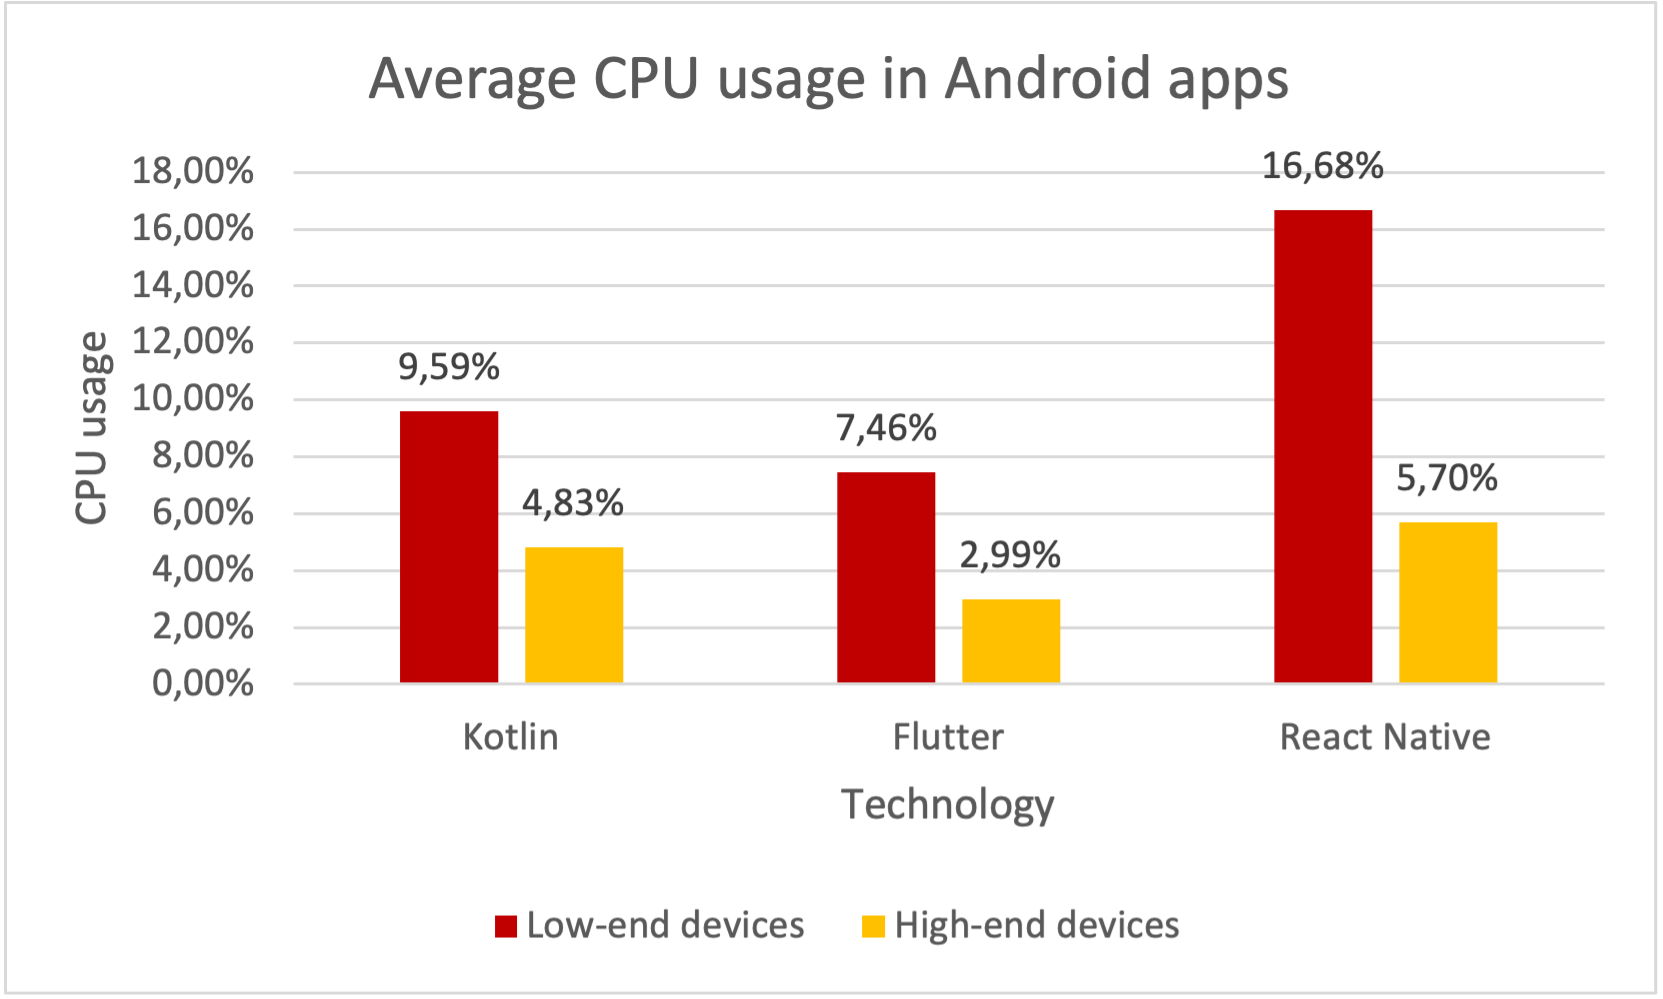
\includegraphics[width=\textwidth]{img/cpu_average_android}
        \caption{Average CPU usage in Android apps (Source: Own work)}
        \label{fig:cpu_avg_android}
    \end{minipage}
    \hfill
    \begin{minipage}{.48\textwidth}
        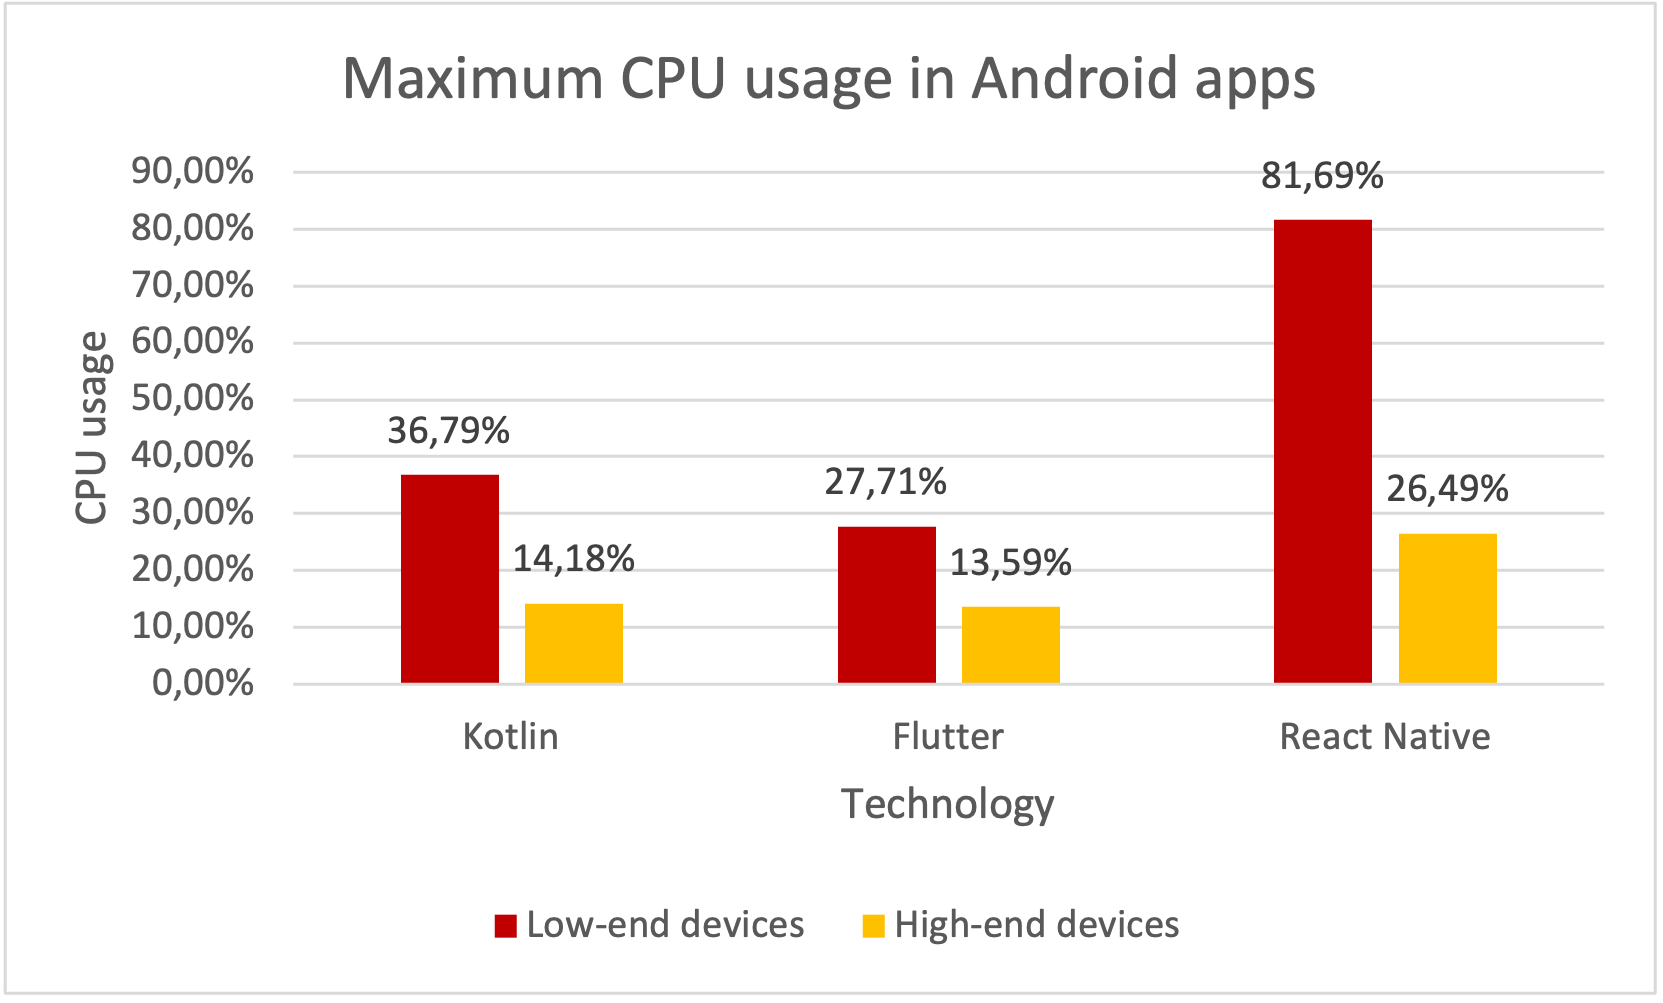
\includegraphics[width=\textwidth]{img/cpu_max_android}
        \caption{Maximum CPU usage in Android apps (Source: Own work)}
        \label{fig:cpu_max_android}
    \end{minipage}
\end{figure}

Figures \ref{fig:cpu_avg_android} and \ref{fig:cpu_max_android} show the comparison of CPU usage among Android apps developed with Kotlin, Flutter, and React Native. Overall, Flutter apps require the least CPU capacity across both low-end and high-end devices, thus implying the most efficient utilization of system resources. Kotlin apps perform slightly worse than Flutter apps, but they still do not exceed even 10\% of CPU usage, which is a great result. React Native apps show the highest CPU usage, most notably on low-end devices. Furthermore, they experience the highest spikes, reaching over 80\%. Such spikes may be concerning if they keep happening regularly. Kotlin and Flutter apps exhibit much lower maximum CPU usage.

\begin{figure}[H]
    \begin{minipage}{.48\textwidth}
        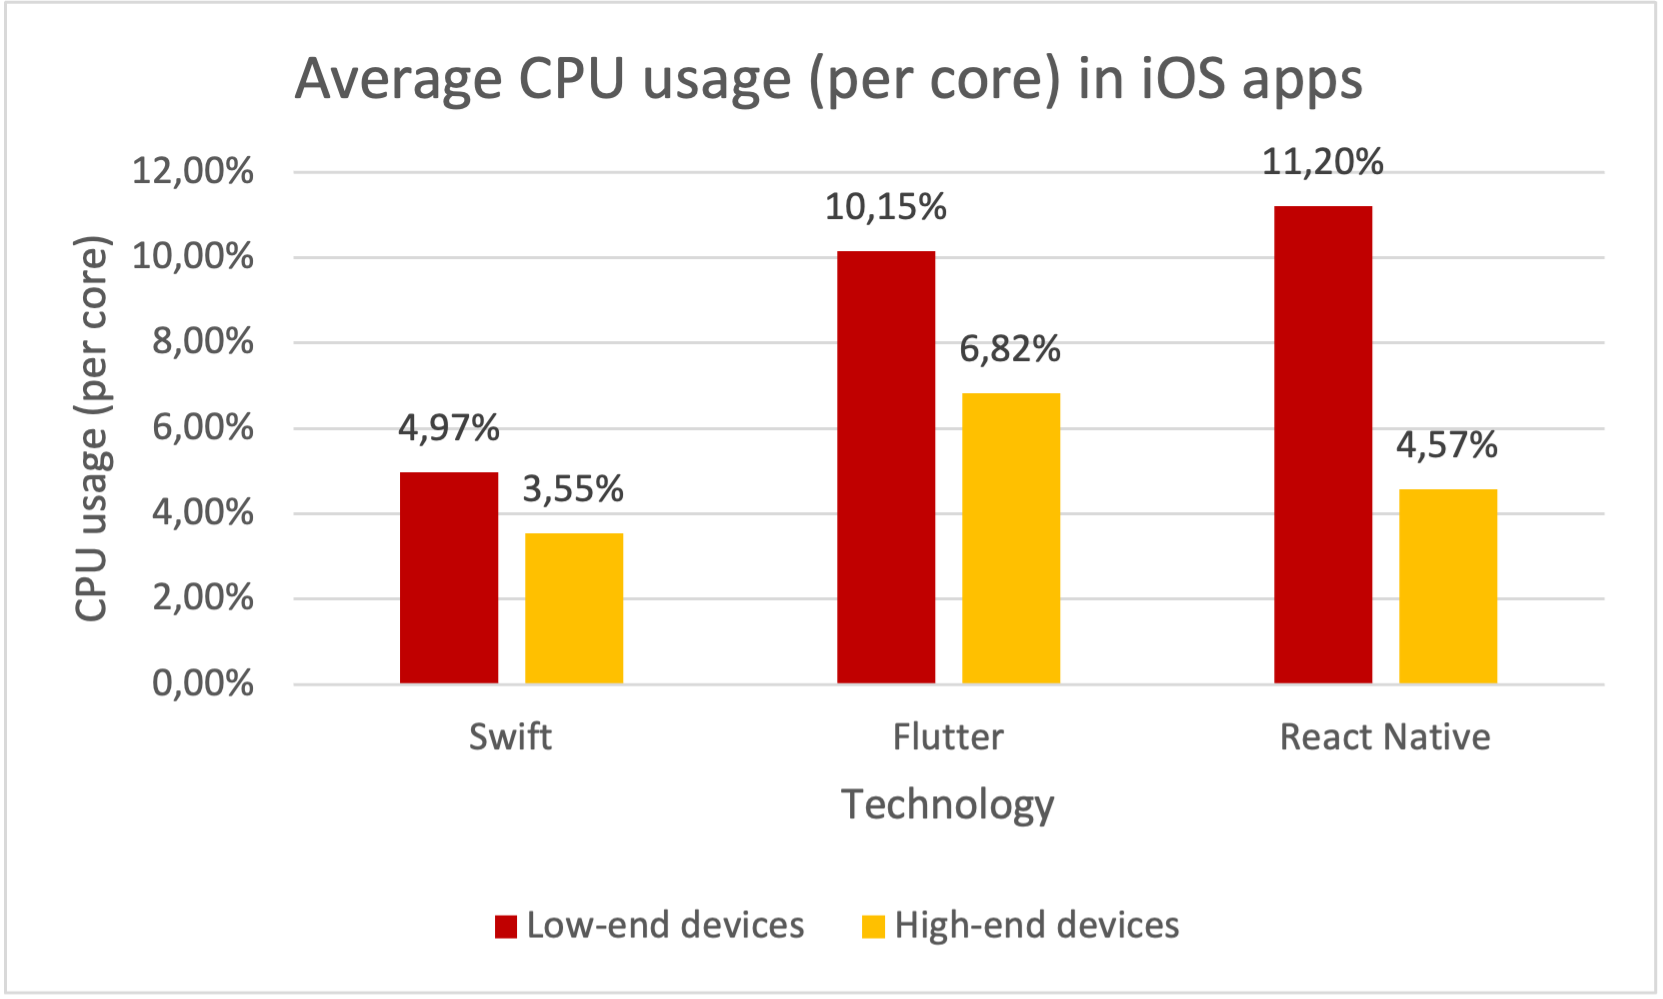
\includegraphics[width=\textwidth]{img/cpu_average_ios}
        \caption{Average CPU usage in iOS apps (Source: Own work)}
        \label{fig:cpu_avg_ios}
    \end{minipage}
    \hfill
    \begin{minipage}{.48\textwidth}
        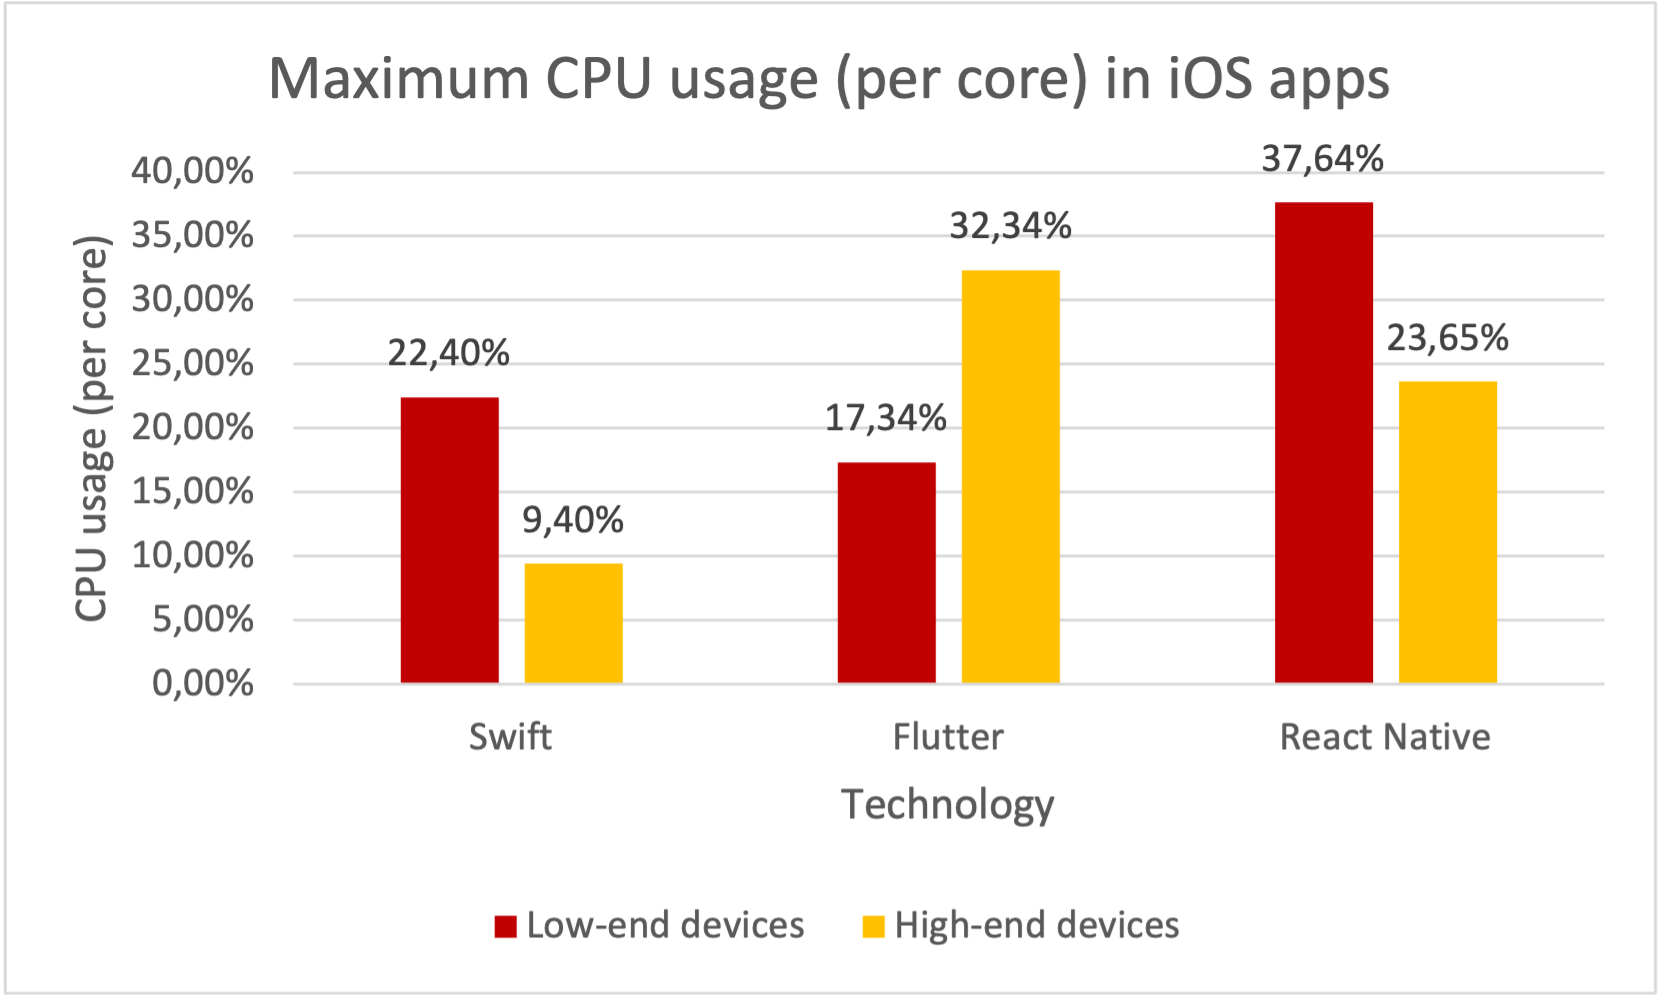
\includegraphics[width=\textwidth]{img/cpu_max_ios}
        \caption{Maximum CPU usage in iOS apps (Source: Own work)}
        \label{fig:cpu_max_ios}
    \end{minipage}
\end{figure}

Figures \ref{fig:cpu_avg_ios} and \ref{fig:cpu_max_ios} show the comparison of CPU usage among iOS apps developed with Swift, Flutter, and React Native. Swift apps perform the best on both low-end and high-end devices, with the average CPU usage remaining just under 5\% per core. Flutter apps and React Native apps exhibit similar results, although the former perform better on low-end devices and the latter perform better on high-end devices. However, React Native apps demonstrate the highest CPU usage spikes, similar to their Android equivalents.

\begin{figure}[H]
    \begin{minipage}{.48\textwidth}
        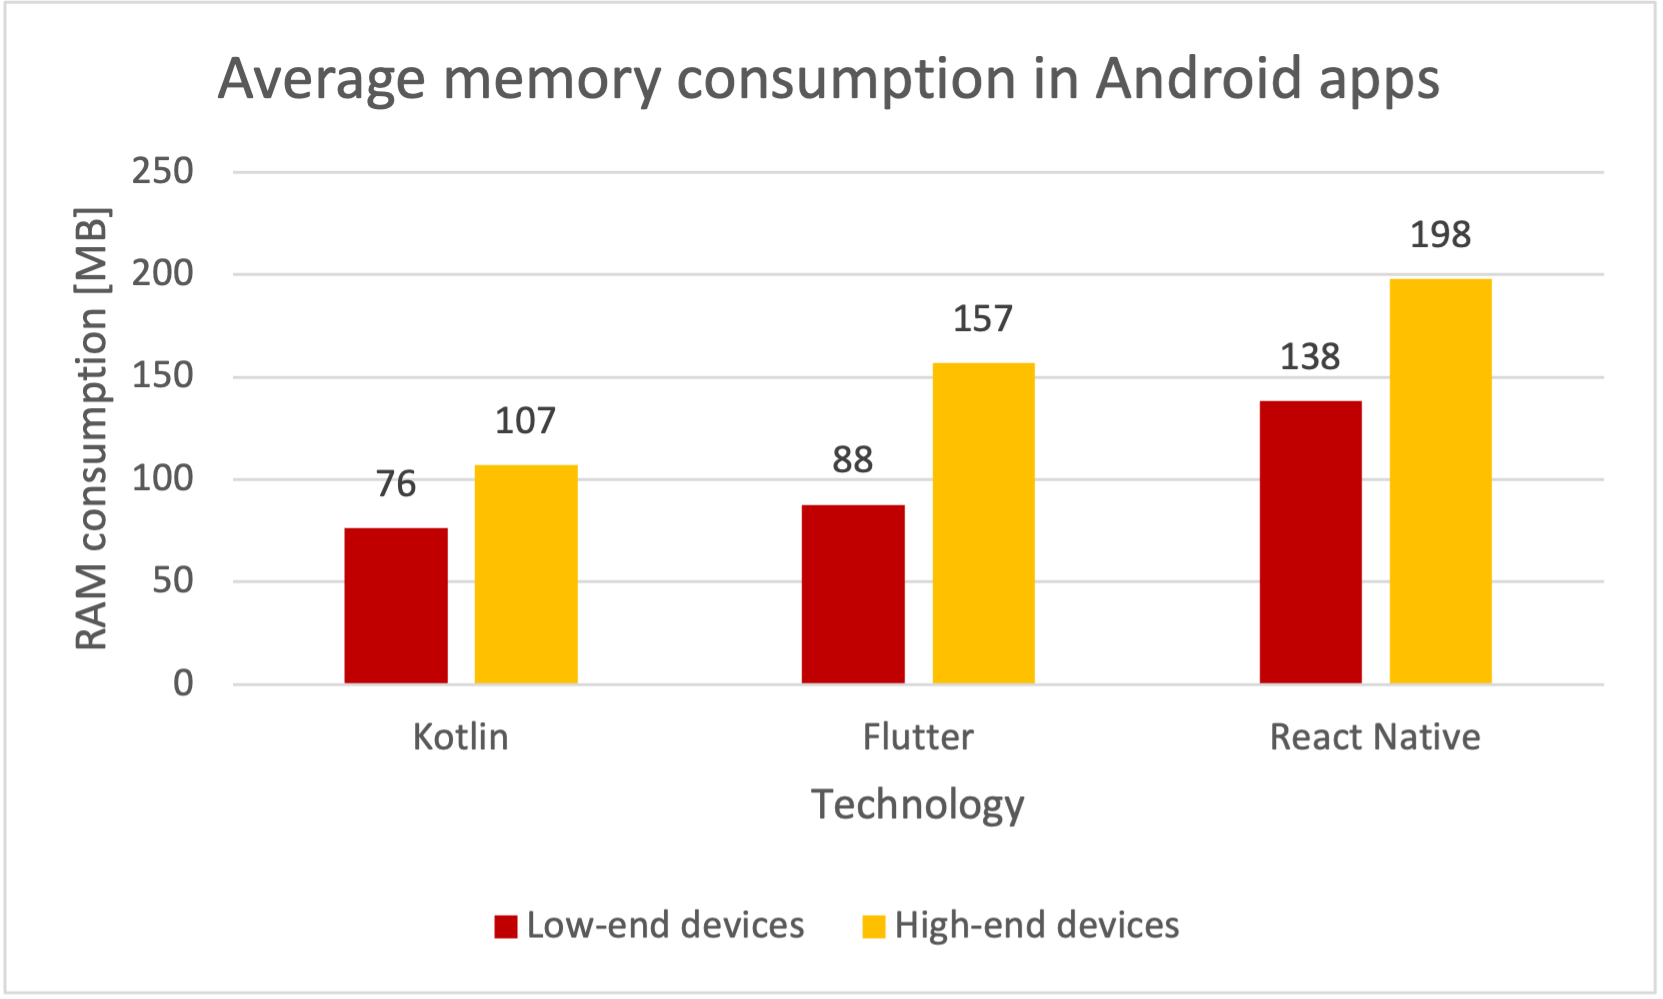
\includegraphics[width=\textwidth]{img/ram_average_android}
        \caption{Average memory consumption in Android apps (Source: Own work)}
        \label{fig:ram_avg_android}
    \end{minipage}
    \hfill
    \begin{minipage}{.48\textwidth}
        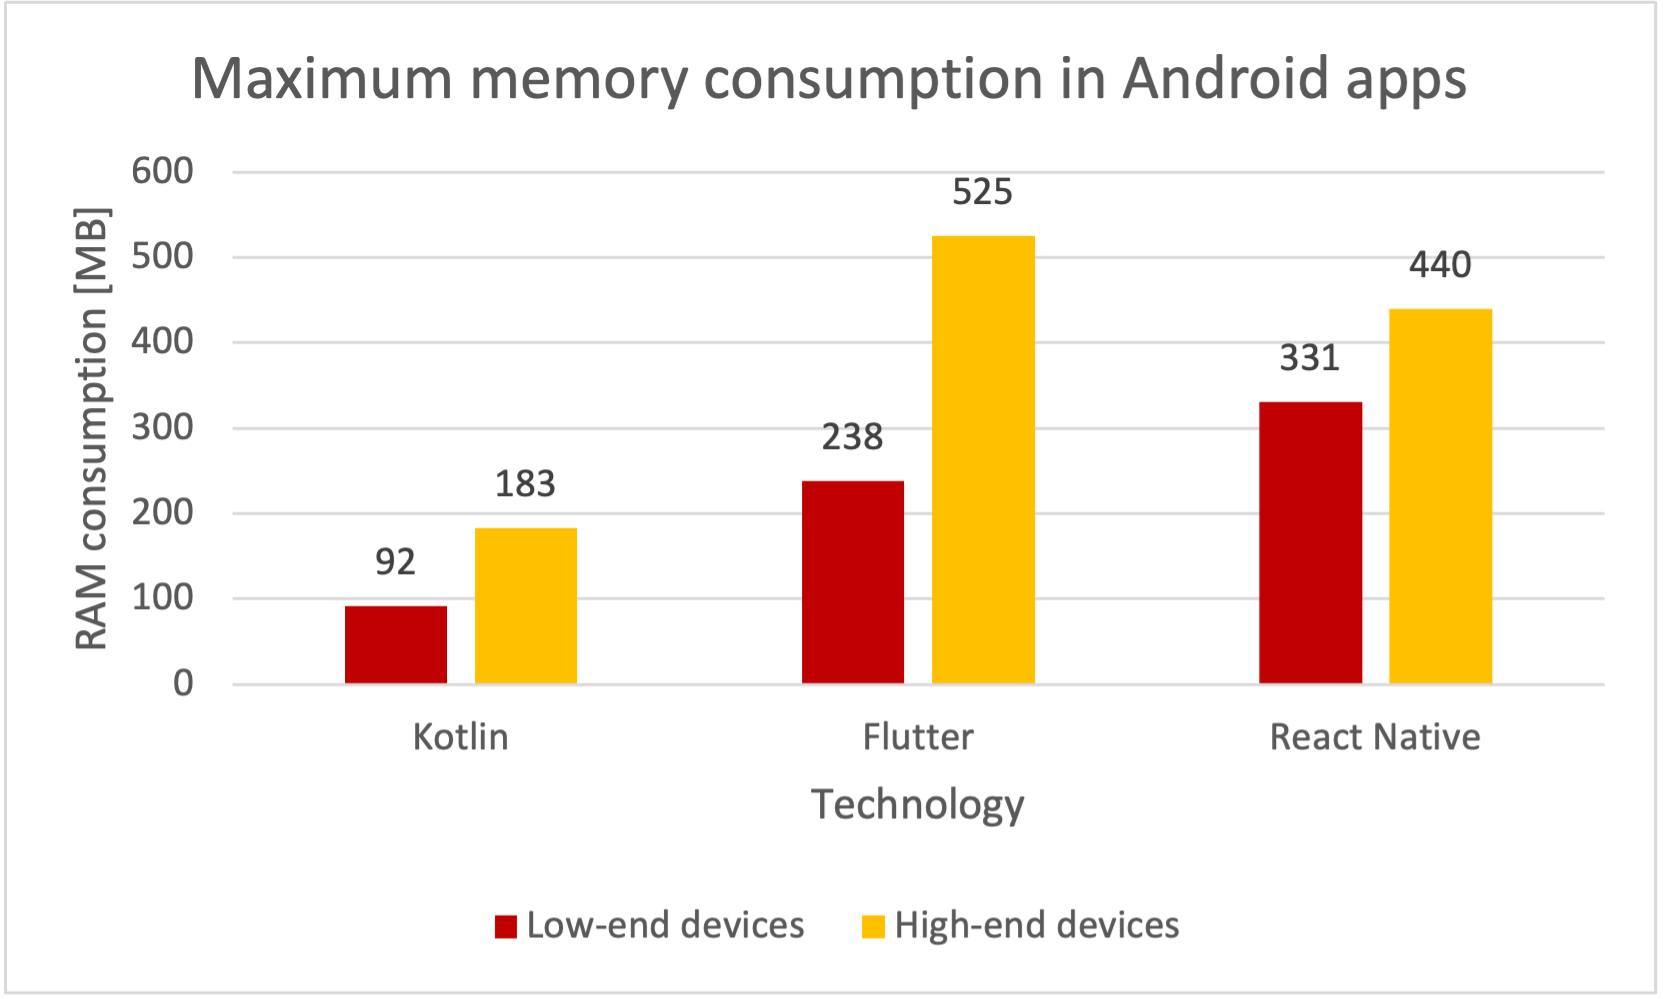
\includegraphics[width=\textwidth]{img/ram_max_android}
        \caption{Maximum memory consumption in Android apps (Source: Own work)}
        \label{fig:ram_max_android}
    \end{minipage}
\end{figure}

Figures \ref{fig:ram_avg_android} and \ref{fig:ram_max_android} show the comparison of memory consumption among Android apps developed with Kotlin, Flutter, and React Native. It can be observed that each technology has a similar ratio of memory used by low-end devices to memory used by high-end devices. Overall, Kotlin apps utilize the least memory resources, followed by Flutter apps, and then React Native apps. However, Flutter apps experience the highest spikes in RAM consumption, with the maximum reaching 525 MB on high-end devices as compared to Kotlin apps 183 MB. Nevertheless, high-end devices currently offer a solid amount of memory; therefore, such values (if sporadic) do not have to mean performance issues. Maximum memory usage should be tracked primarily on low-end devices.

\begin{figure}[H]
    \begin{minipage}{.48\textwidth}
        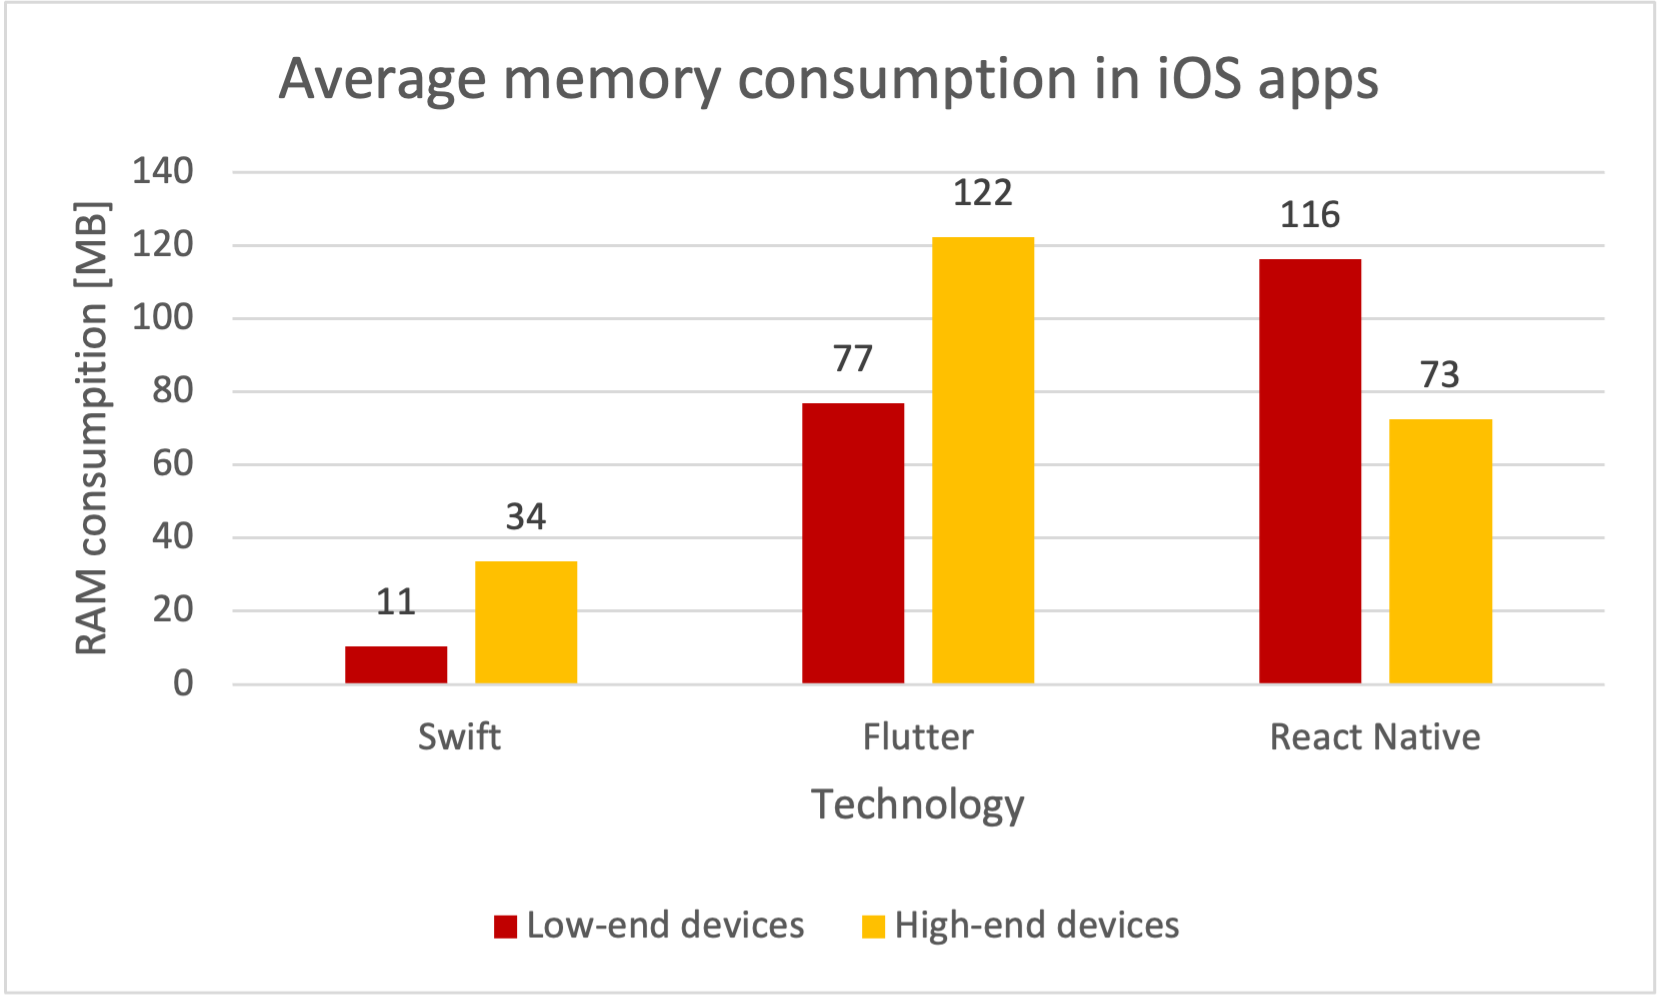
\includegraphics[width=\textwidth]{img/ram_average_ios}
        \caption{Average memory consumption in iOS apps (Source: Own work)}
        \label{fig:ram_avg_ios}
    \end{minipage}
    \hfill
    \begin{minipage}{.48\textwidth}
        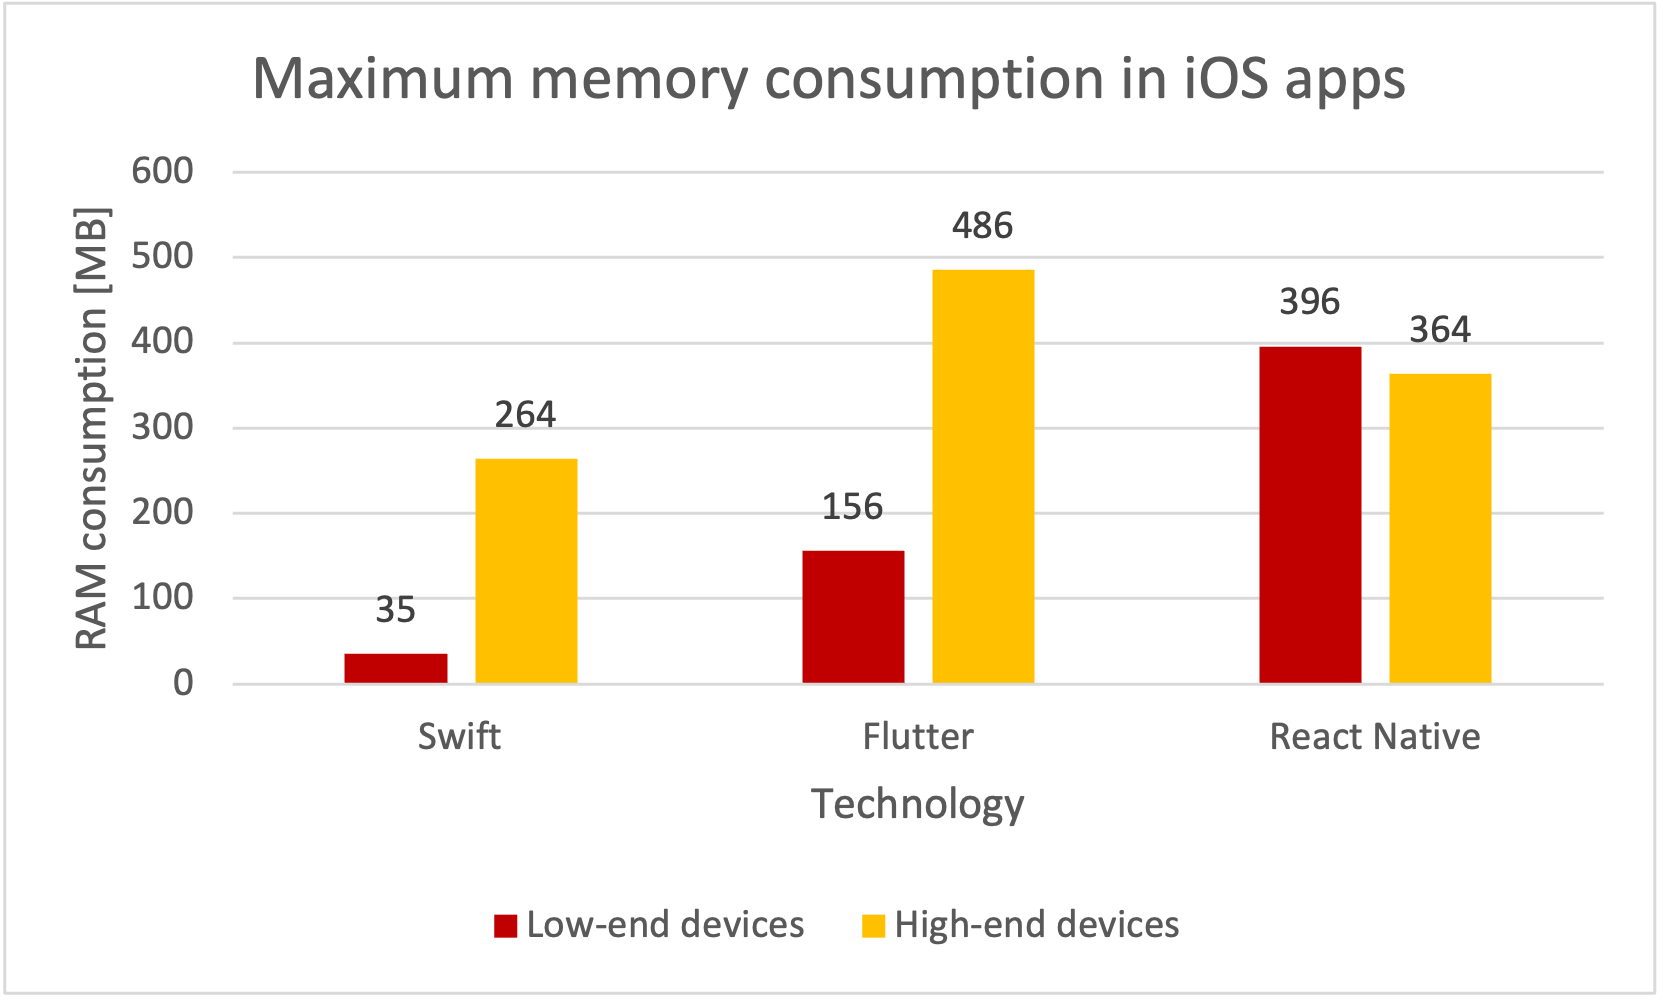
\includegraphics[width=\textwidth]{img/ram_max_ios}
        \caption{Maximum memory consumption in iOS apps (Source: Own work)}
        \label{fig:ram_max_ios}
    \end{minipage}
\end{figure}

Figures \ref{fig:ram_avg_ios} and \ref{fig:ram_max_ios} show the comparison of memory consumption among iOS apps developed with Swift, Flutter, and React Native. Swift apps exhibit considerably lower memory consumption compared to the other technologies. For low-end devices, Flutter performs moderately better than React Native. On the other hand, React Native apps utilize less memory on high-end devices than Flutter apps. Again, Flutter is responsible for the highest spikes on high-end devices.

\begin{figure}[H]
    \begin{minipage}{.48\textwidth}
        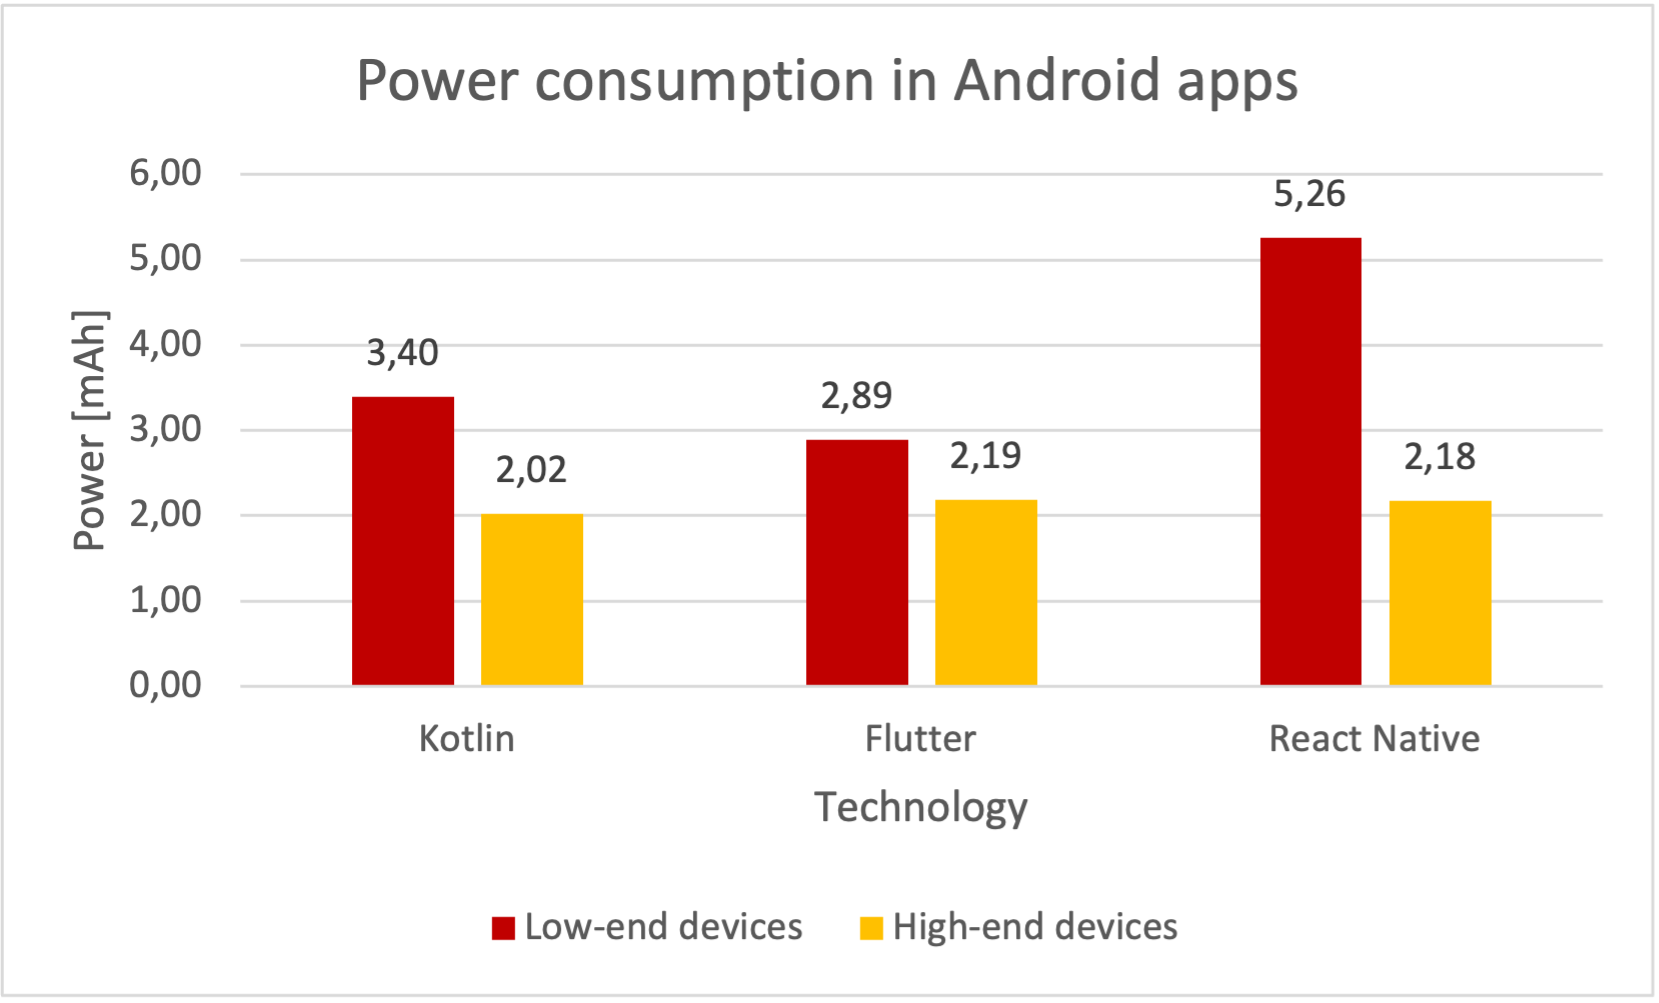
\includegraphics[width=\textwidth]{img/power_android}
        \caption{Power consumption in Android apps (Source: Own work)}
        \label{fig:power_android}
    \end{minipage}
    \hfill
    \begin{minipage}{.48\textwidth}
        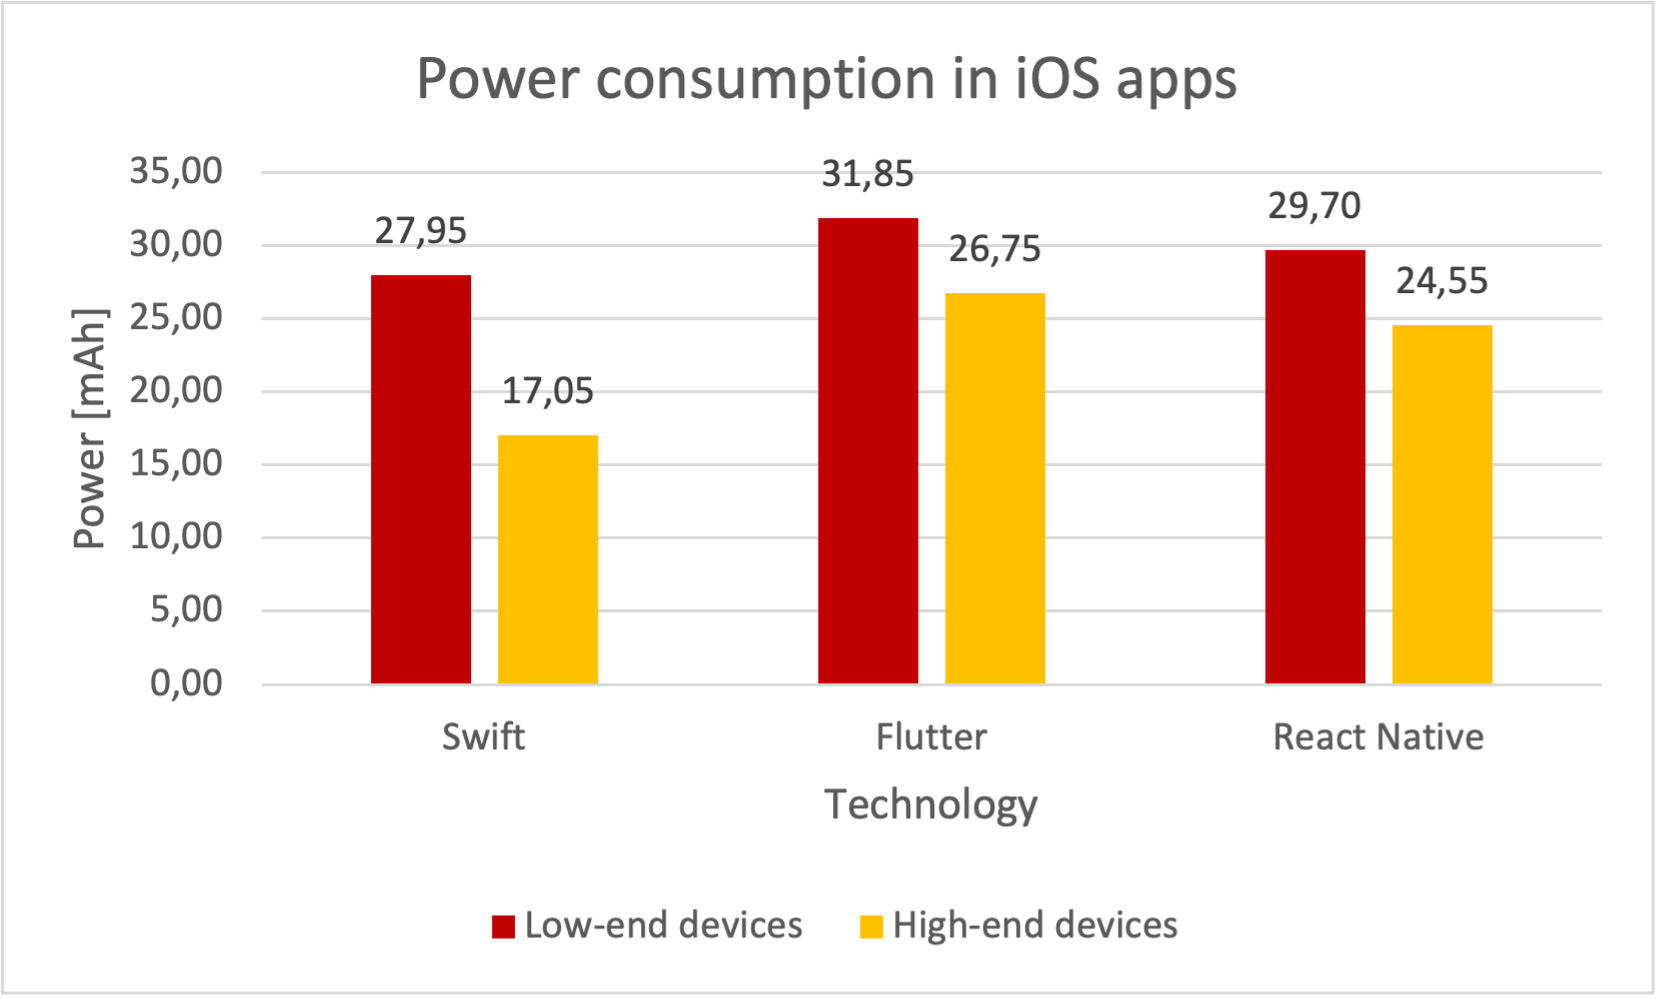
\includegraphics[width=\textwidth]{img/power_ios}
        \caption{Power consumption in iOS apps (Source: Own work)}
        \label{fig:power_ios}
    \end{minipage}
\end{figure}

Figures \ref{fig:power_android} and \ref{fig:power_ios} show the comparison of power consumption among Android and iOS apps developed with Kotlin, Flutter, Swift, and React Native. Overall, Android apps perform similarly on high-end devices. Considering power consumption on low-end devices, Flutter handles it the best. Although the values themselves are really low, the experiment was only carried out for a duration of one minute; therefore, with real-life usage, those values would be further apart. In the case of iOS apps, the results are quite close, apart from Swift apps that perform noticeably better on high-end devices.

\begin{figure}[H]
    \begin{minipage}{.48\textwidth}
        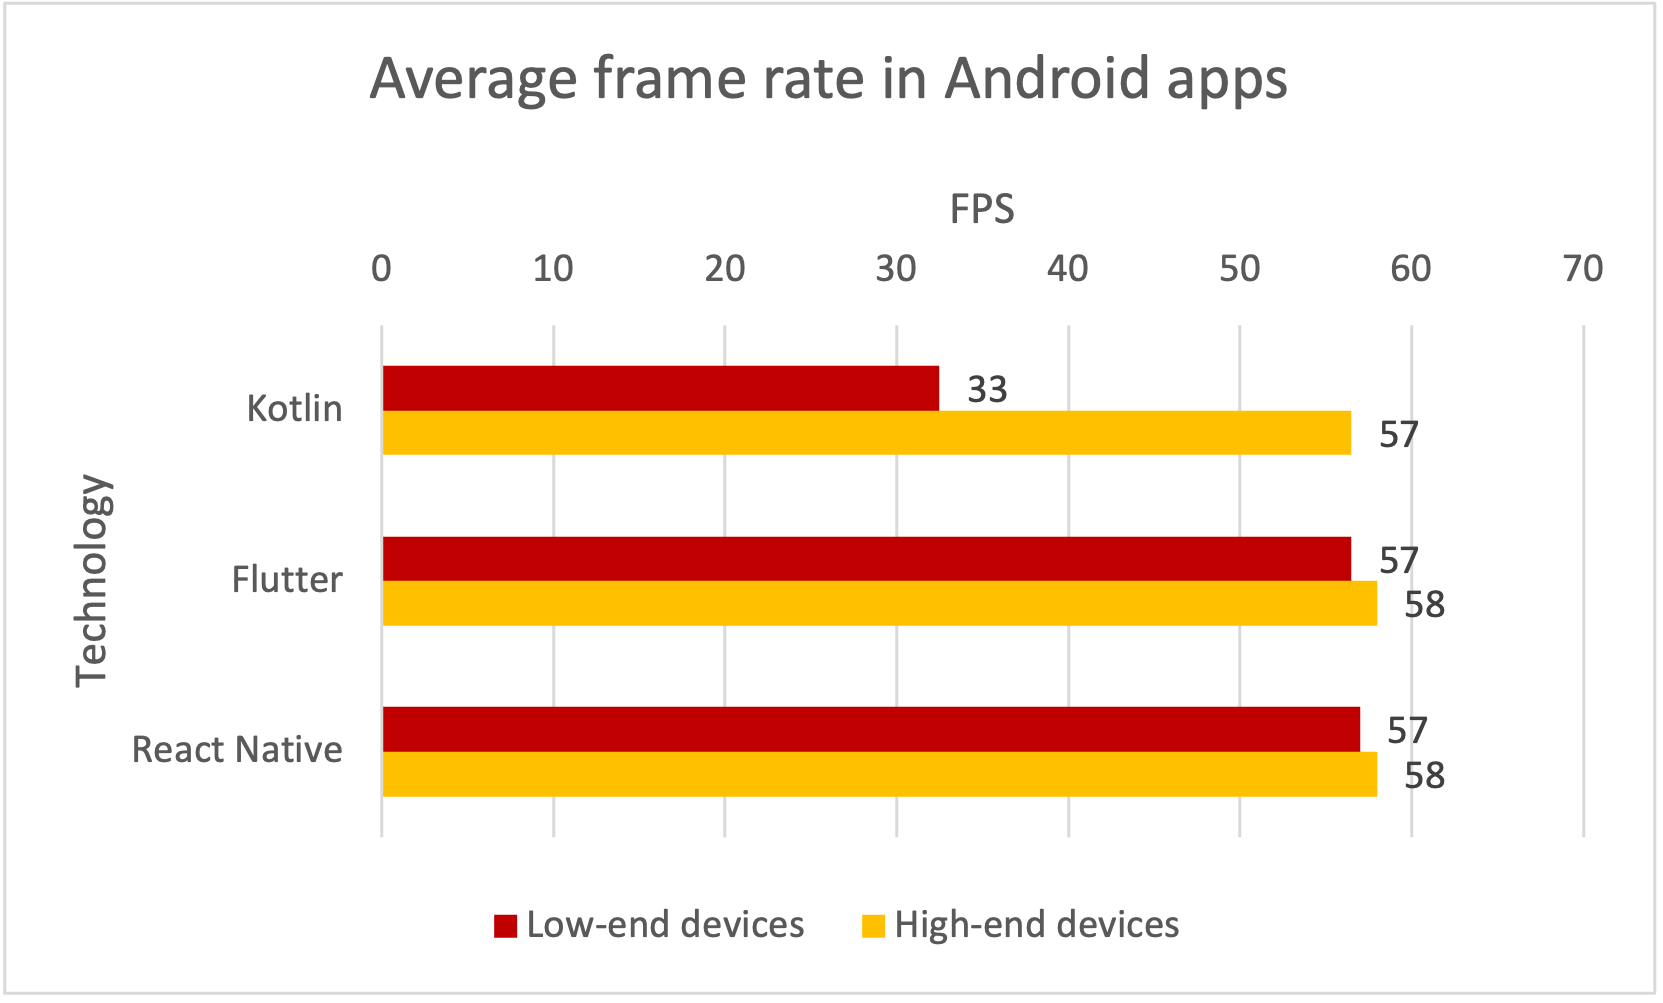
\includegraphics[width=\textwidth]{img/fps_average_android}
        \caption{Average frame rate in Android apps (Source: Own work)}
        \label{fig:fps_avg_android}
    \end{minipage}
    \hfill
    \begin{minipage}{.48\textwidth}
        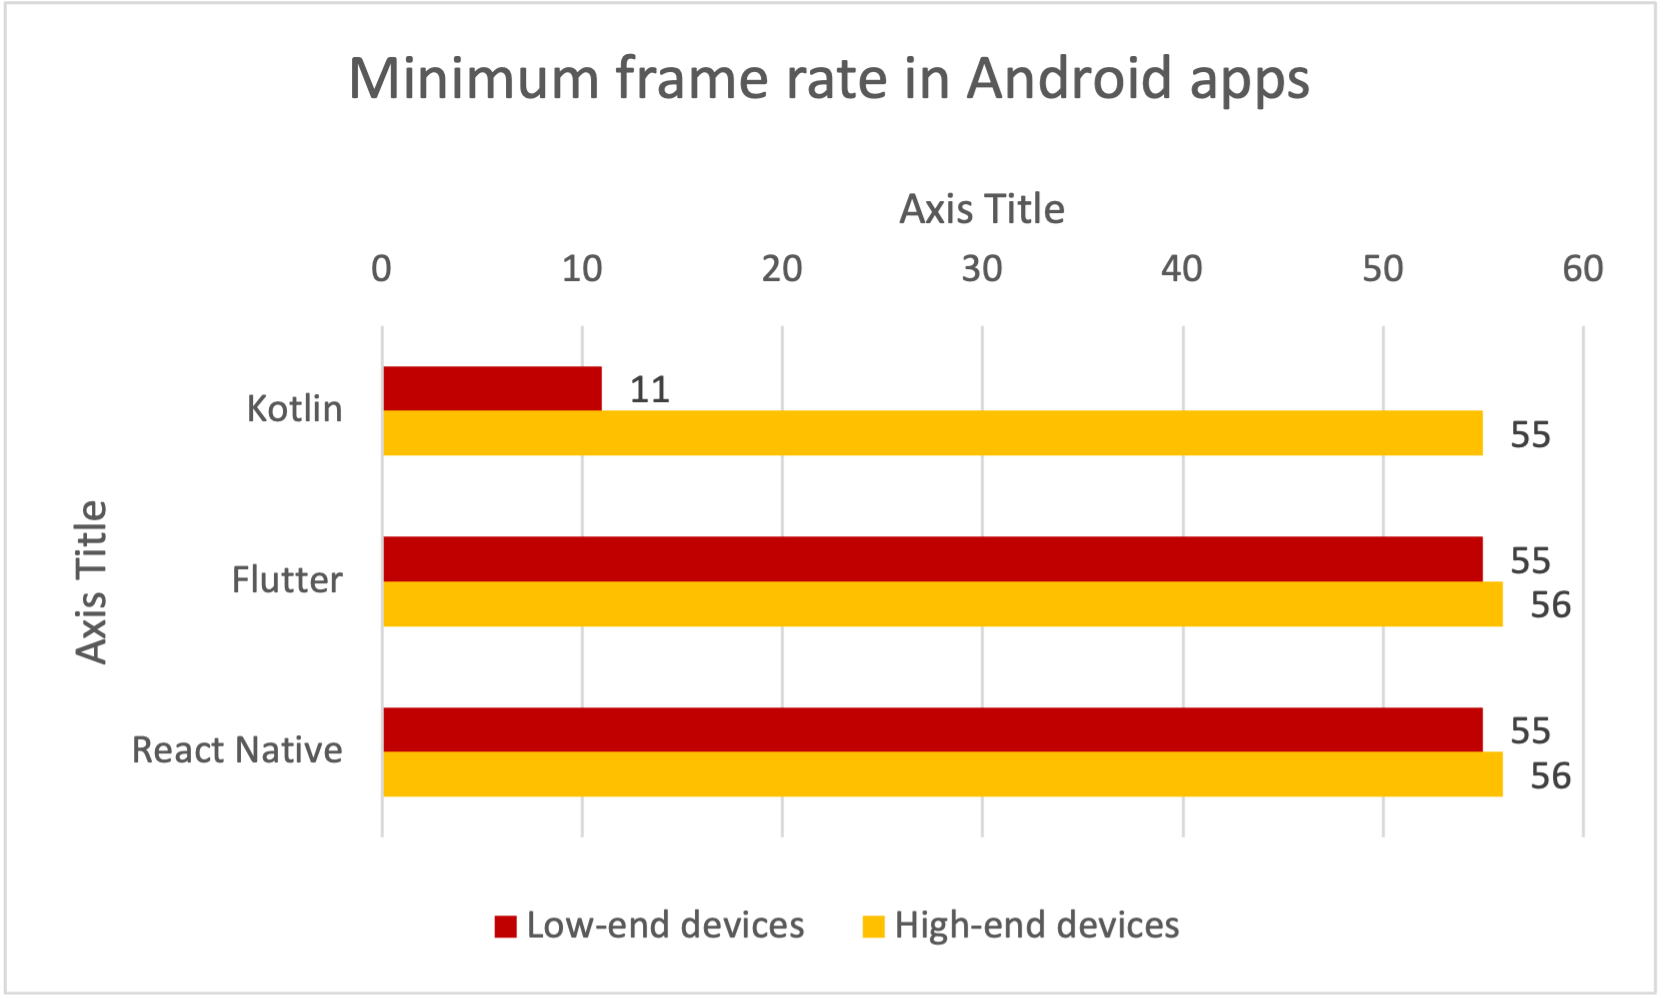
\includegraphics[width=\textwidth]{img/fps_min_android}
        \caption{Minimum frame rate in Android apps (Source: Own work)}
        \label{fig:fps_min_android}
    \end{minipage}
\end{figure}

Figures \ref{fig:fps_avg_android} and \ref{fig:fps_min_android} show the comparison of frame rate among Android apps developed with Kotlin, Flutter, and React Native. For high-end devices, there are no significant differences in the smoothness of apps developed with either technology. The range of 55--58 FPS on average is considered to be an excellent result. However, Kotlin apps struggle on low-end devices, experiencing 10 FPS drops and an average frame rate of 33 FPS. Flutter and React Native apps achieve similarly good results on low-end and high-end devices.

\begin{figure}[H]
    \begin{minipage}{.48\textwidth}
        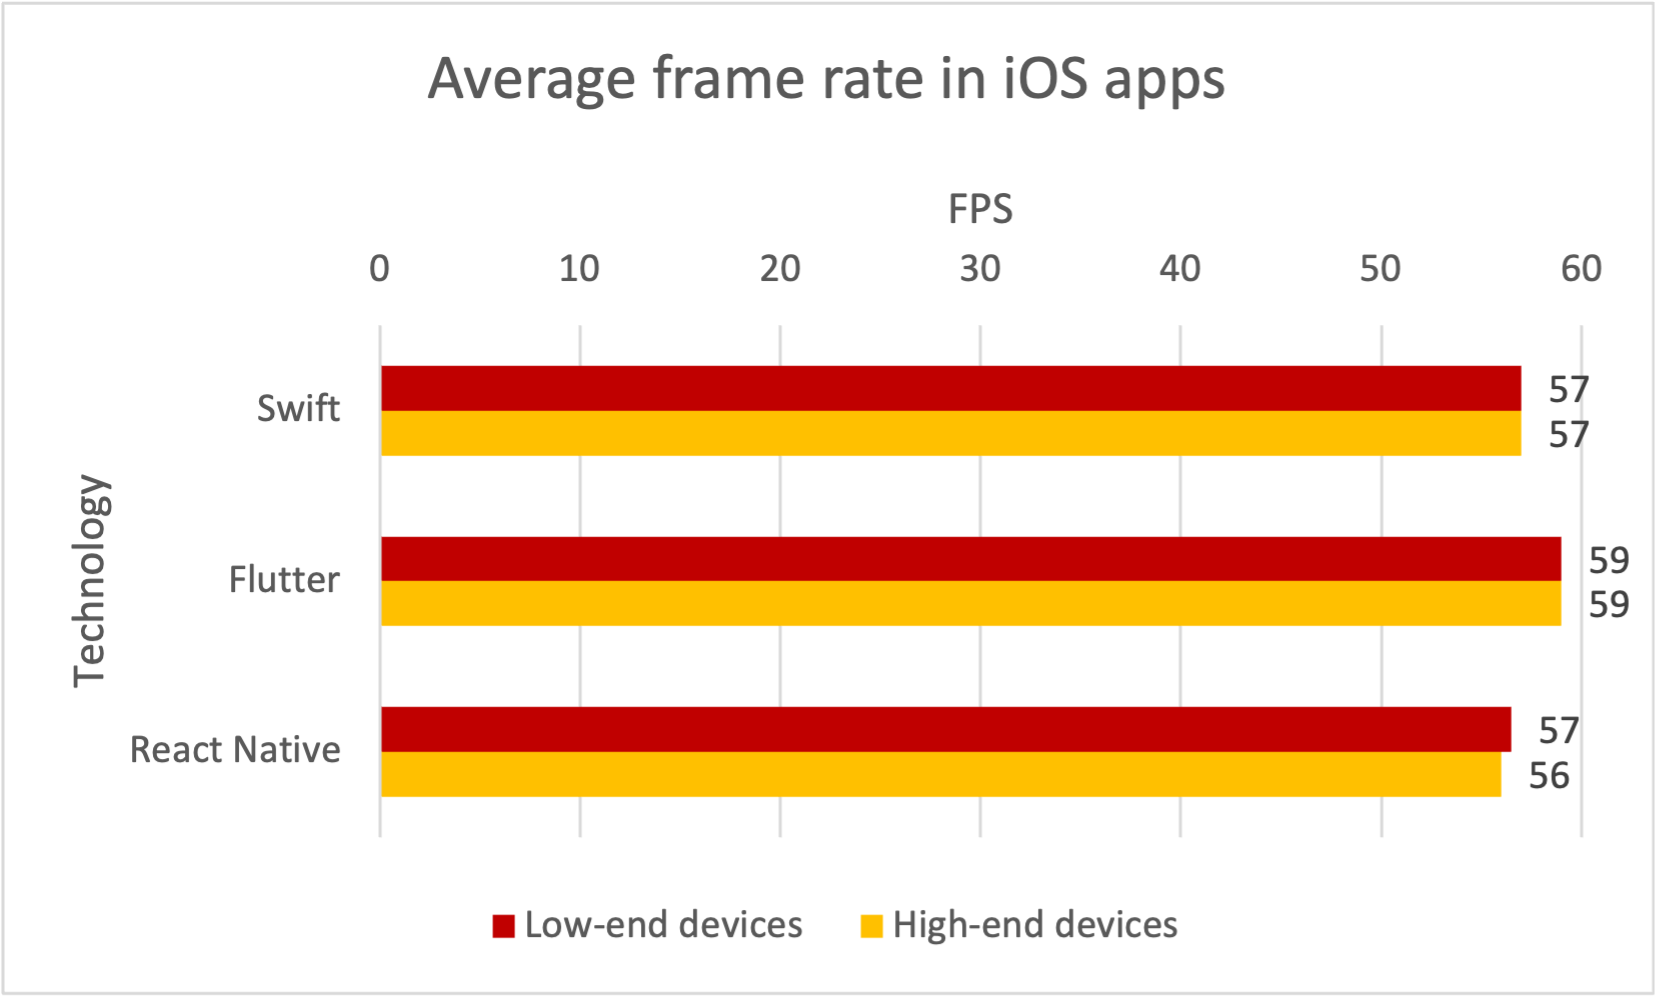
\includegraphics[width=\textwidth]{img/fps_average_ios}
        \caption{Average frame rate in iOS apps (Source: Own work)}
        \label{fig:fps_avg_ios}
    \end{minipage}
    \hfill
    \begin{minipage}{.48\textwidth}
        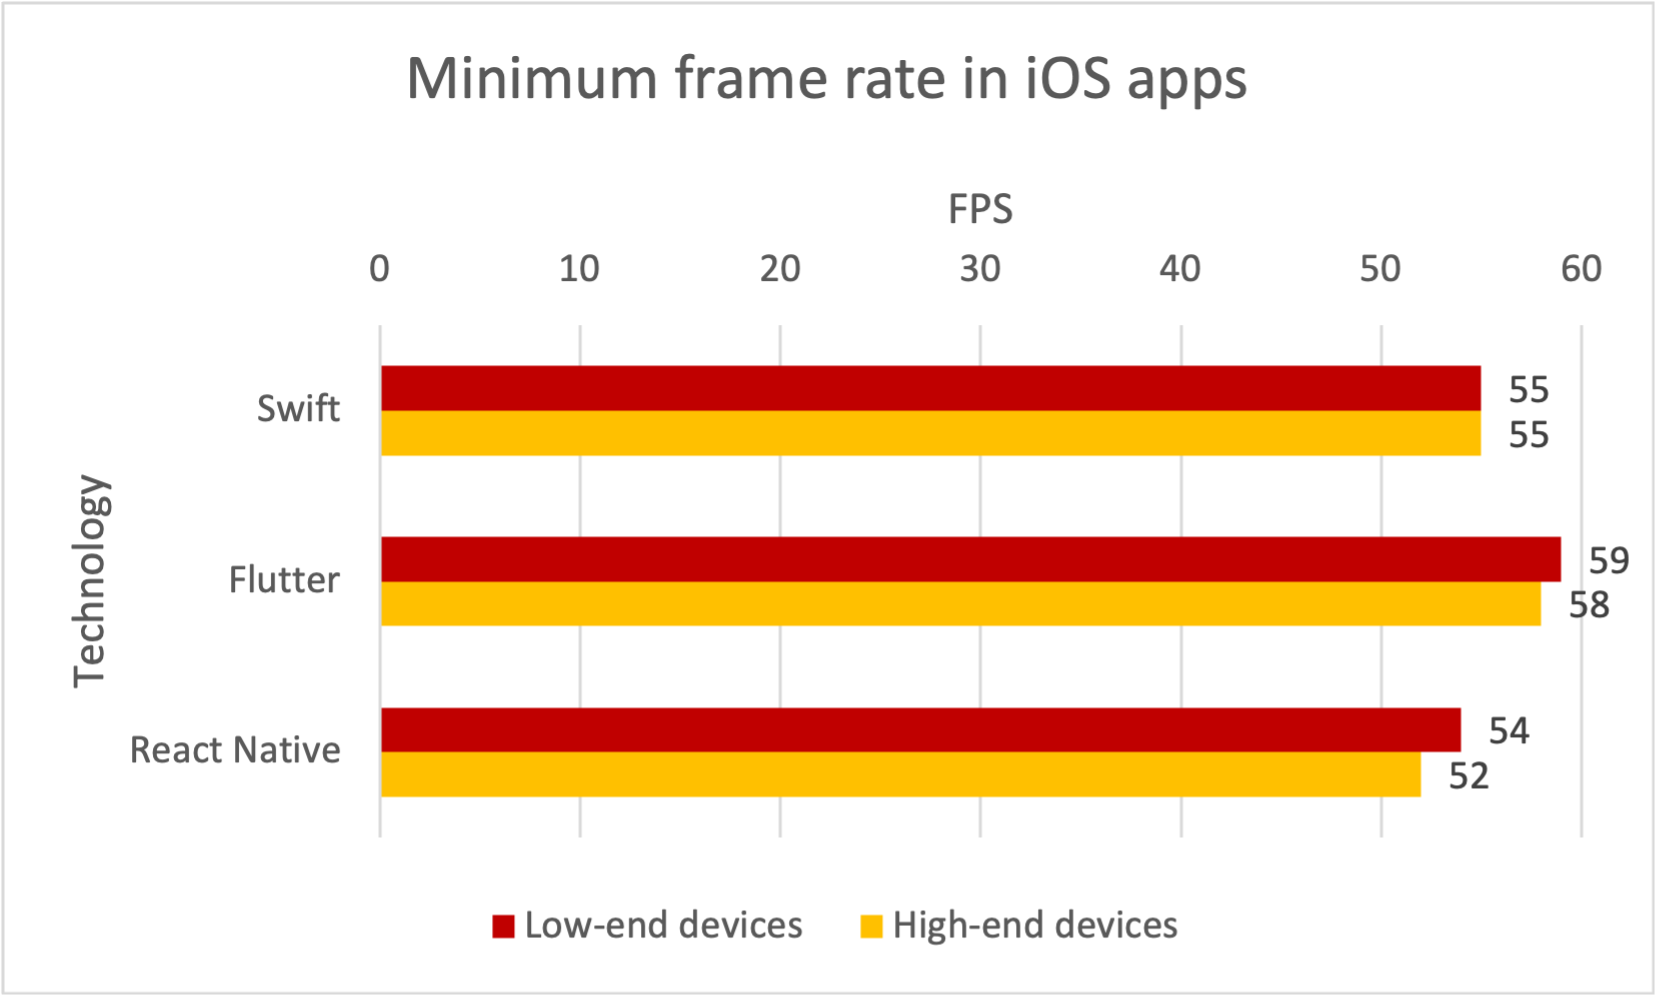
\includegraphics[width=\textwidth]{img/fps_min_ios}
        \caption{Minimum frame rate in iOS apps (Source: Own work)}
        \label{fig:fps_min_ios}
    \end{minipage}
\end{figure}

Figures \ref{fig:fps_avg_ios} and \ref{fig:fps_min_ios} show the comparison of frame rate among iOS apps developed with Swift, Flutter, and React Native. Overall, Flutter apps exhibit the highest frame rate of 59 FPS on low-end and high-end devices. Swift and React Native apps demonstrate 56--57 FPS frame rate on average. No significant FPS drops can be observed, with React Native apps experiencing a minimum of 52 FPS on high-end devices.

\begin{figure}[H]
    \begin{minipage}{.48\textwidth}
        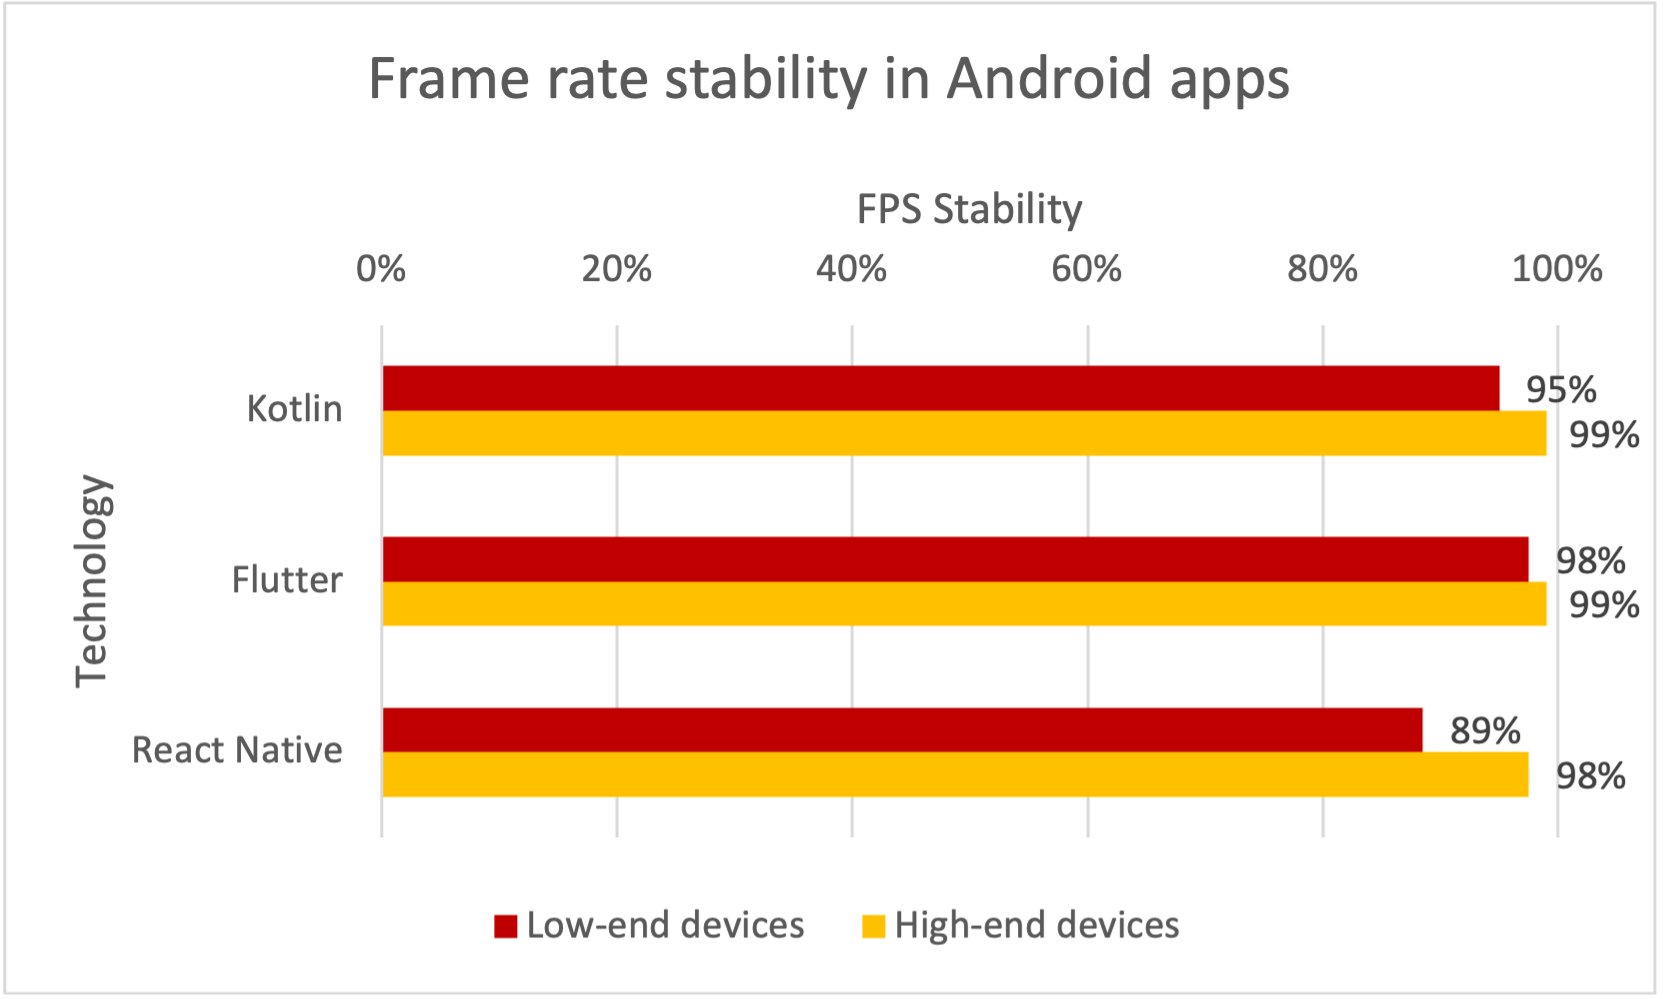
\includegraphics[width=\textwidth]{img/fps_stability_android}
        \caption{Frame rate stability in Android apps (Source: Own work)}
        \label{fig:fps_stability_android}
    \end{minipage}
    \hfill
    \begin{minipage}{.48\textwidth}
        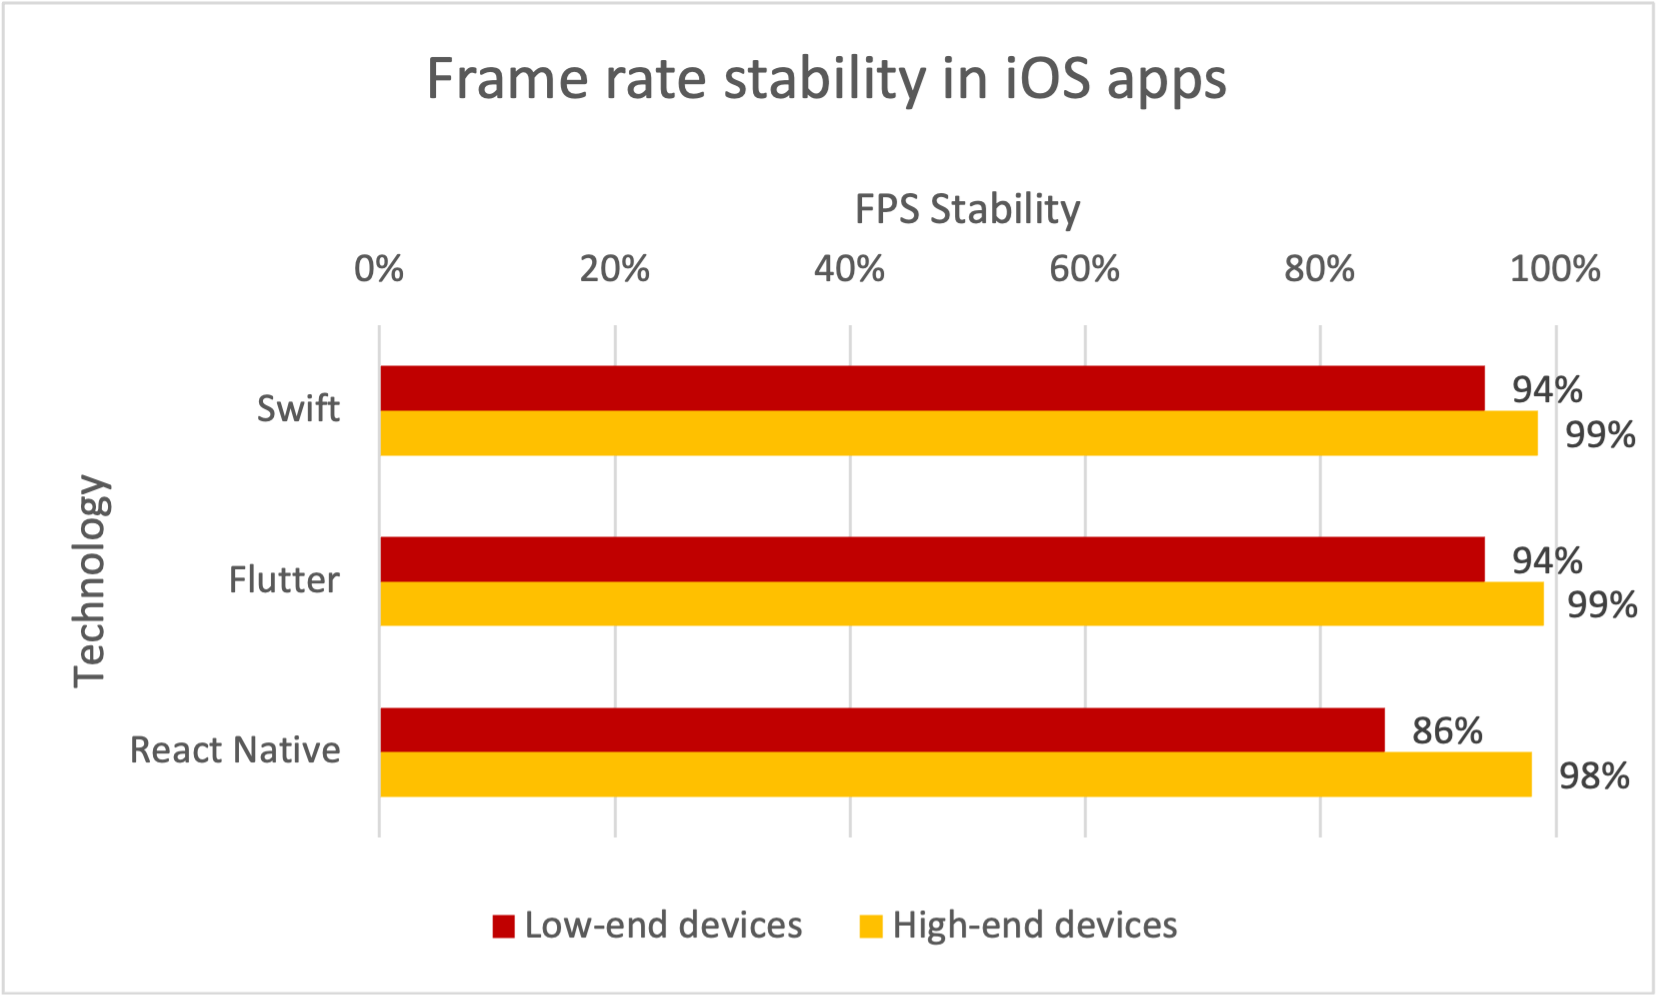
\includegraphics[width=\textwidth]{img/fps_stability_ios}
        \caption{Frame rate stability in iOS apps (Source: Own work)}
        \label{fig:fps_stability_ios}
    \end{minipage}
\end{figure}

Figures \ref{fig:fps_stability_android} and \ref{fig:fps_stability_ios} show the comparison of frame rate stability among Android and iOS apps developed with Kotlin, Swift, Flutter, and React Native. The results are closely comparable, considering either platform. On both low-end and high-end devices, each technology offers high frame rate stability. Only React Native apps installed on low-end devices experience stability below 90\%.
